\documentclass[../main.tex]{subfiles}
\graphicspath{{\subfix{../images/}}} % Pfad zu den Bilddateien anpassen

\begin{document}

% ==============================================
% LATEX TEMPLATE TUTORIAL
% BA Bautzen Wirtschaft - Alle Custom Commands
% ==============================================

\section{LaTeX Template Tutorial}

Dieses Dokument zeigt alle verfügbaren benutzerdefinierten Befehle und Features.

% ==============================================
% GRUNDLEGENDE TEXTFORMATIERUNG
% ==============================================

\subsection{Grundlegende Textformatierung}

\textbf{Fettgedruckter Text} mit \verb|\textbf{}|\\
\textit{Kursiver Text} mit \verb|\textit{}|\\
\underline{Unterstrichener Text} mit \verb|\underline{}|

% ==============================================
% ZITIERWEISE (CHICAGO STYLE)
% ==============================================

\subsection{Zitierweise - Chicago Manual of Style}

Standard-Zitierung: \autocite{smith2018}\\
Mit Seitenzahl: \autocite[42]{smith2018}\\
Mehrere Seiten: \autocite[15-27]{johnson2020}\\
Mehrere Quellen: \autocite{smith2018}, \autocite{johnson2020}

% Gesetzeszitate (spezielle Syntax)
Gesetzeszitat: \lawcite[§ 164 Absatz 1 Satz 1]{aktg1965}

% ==============================================
% ABKÜRZUNGEN UND GLOSSAR
% ==============================================

\subsection{Abkürzungen und Glossar}

Erste Verwendung (ausgeschrieben): \gls{ai}\\
Zweite Verwendung (abgekürzt): \gls{ai}\\
Weitere Abkürzungen: \gls{ml}, \gls{dl}

% Abkürzungen werden in build/acronyms/acronyms.tex definiert:
% \newacronym{ai}{AI}{Artificial Intelligence}

% ==============================================
% ABBILDUNGEN UND TABELLEN
% ==============================================

\subsection{Abbildungen}

\begin{figure}[h]
    \centering
    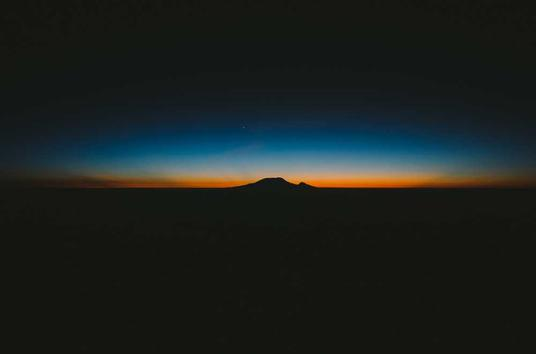
\includegraphics[width=4cm]{images/picsum lorem.jpg}
    \caption{Beispiel-Abbildung mit korrekter BA Bautzen Formatierung}
    \label{fig:tutorial_image}
\end{figure}

Verweis auf Abbildung: \cref{fig:tutorial_image}

\subsection{Tabellen}

\begin{table}[h]
    \centering
    \begin{tabular}{|c|c|c|}
        \hline
        \textbf{Spalte 1} & \textbf{Spalte 2} & \textbf{Spalte 3} \\
        \hline
        Wert A & Wert B & Wert C \\
        Wert D & Wert E & Wert F \\
        \hline
    \end{tabular}
    \caption{Beispiel-Tabelle nach BA Bautzen Standards}
    \label{tab:tutorial_table}
\end{table}

Verweis auf Tabelle: \cref{tab:tutorial_table}

% ==============================================
% DEFINITIONEN
% ==============================================

\subsection{Definitionen}

\begin{definition}
Eine \textbf{Definition} ist eine genaue Bestimmung eines Begriffes durch Angabe seiner wesentlichen Merkmale.
\end{definition}

% ==============================================
% TODO-FUNKTIONALITÄT
% ==============================================

\subsection{TODO-Funktionalität}

Verschiedene TODO-Typen:
\todo{Das ist ein normales TODO}
\idea{Das ist eine Idee für später}
\critical{Das ist eine kritische Aufgabe}

TODO-Liste:
\begin{todolist}
    \item \todo{Erste Aufgabe erledigen}
    \item \idea{Neue Idee ausarbeiten}
    \item \critical{Kritisches Problem lösen}
\end{todolist}

% Alle TODOs anzeigen mit: \printtodos (normalerweise am Ende des Dokuments)
% TODOs verstecken mit: \hideTodos (in main.tex)

% ==============================================
% KI-KENNZEICHNUNG (Neue englische Befehle)
% ==============================================

\subsection{KI-Kennzeichnung nach BA Bautzen Richtlinien}

\textbf{Wichtig:} KI muss mit \verb|\enableAI| in main.tex aktiviert werden!

\subsubsection{Fußnoten-Kennzeichnung}
Dieser Textabschnitt wurde mit KI erstellt.
\aifootnote{ChatGPT 4.0}{Erkläre die Grundlagen des Marketings}{15.03.2024}

\subsubsection{Inline-Kennzeichnung}
\aisection{Claude 3.5}{Erstelle eine Marktanalyse für E-Commerce}{16.03.2024}
Dieser Abschnitt wurde mit KI-Unterstützung verfasst.

\subsubsection{Vollständiger Absatz}
\aiparagraph{ChatGPT 4.0}{Schreibe einen Absatz über Digitalisierung}{17.03.2024}
Die Digitalisierung verändert unsere Arbeitswelt fundamental. Neue Technologien ermöglichen effizientere Prozesse und schaffen gleichzeitig neue Herausforderungen für Unternehmen.

\subsubsection{Weitere KI-Befehle}
Tabelle erstellt: \aitable{Excel Copilot}{Erstelle eine Umsatztabelle}{18.03.2024}

Code generiert: \aicode{GitHub Copilot}{Python Funktion für Datenanalyse}{19.03.2024}

Text übersetzt: \aitranslation{DeepL}{Übersetze Abstract ins Englische}{20.03.2024}

Zusammenfassung: \aisummary{ChatGPT 4.0}{Fasse Kapitel 3 zusammen}{21.03.2024}

% ==============================================
% MATHEMATISCHE FORMELN
% ==============================================

\subsection{Mathematische Formeln}

Inline-Formel: $E = mc^2$

Block-Formel:
$$\int_{a}^{b} f(x) \, dx = F(b) - F(a)$$

Nummerierte Gleichung:
\begin{equation}
    \frac{d}{dx}(x^n) = nx^{n-1}
    \label{eq:power_rule}
\end{equation}

Verweis auf Gleichung: \cref{eq:power_rule}

% ==============================================
% LISTEN
% ==============================================

\subsection{Listen}

\textbf{Aufzählung (Punkte):}
\begin{itemize}
    \item Erster Punkt
    \item Zweiter Punkt
    \item Dritter Punkt
\end{itemize}

\textbf{Nummerierte Liste:}
\begin{enumerate}
    \item Erster Schritt
    \item Zweiter Schritt
    \item Dritter Schritt
\end{enumerate}

% ==============================================
% SPEZIELLE UMGEBUNGEN
% ==============================================

\subsection{Spezielle Template-Features}

\textbf{Attachment-Umgebung:}
Wird automatisch für Anlagen verwendet (siehe Ende des Dokuments)

\textbf{Custom List Environment:}
Wird in Anlagen für formatierte Listen verwendet

\textbf{Automatische Verzeichnisse:}
\begin{itemize}
    \item Inhaltsverzeichnis: \verb|\tableofcontents|
    \item Abbildungsverzeichnis: \verb|\listoffigures|
    \item Tabellenverzeichnis: \verb|\listoftables|
    \item Abkürzungsverzeichnis: \verb|\printglossary[type=\acronymtype]|
    \item Anlagenverzeichnis: \verb|\listofattachments|
    \item TODO-Liste: \verb|\printtodos|
    \item KI-Details: \verb|\printailist| (automatisch)
\end{itemize}

% ==============================================
% BIBLIOGRAFIE
% ==============================================

\subsection{Bibliografie-Einstellungen}

\textbf{Drei separate .bib Dateien:}
\begin{itemize}
    \item \verb|references.bib| - Normale Literatur
    \item \verb|law.bib| - Gesetze und Rechtsquellen  
    \item \verb|misc.bib| - Sonstige Quellen
\end{itemize}

\textbf{Ausgabe:}
\begin{itemize}
    \item Quellenverzeichnis: \verb|\printbibliography[notkeyword=law]|
    \item Rechtsquellenverzeichnis: \verb|\printbibliography[keyword=law]|
\end{itemize}

% ==============================================
% KONFIGURATION
% ==============================================

\subsection{Template-Konfiguration}

\textbf{In main.tex anpassen:}
\begin{verbatim}
\title{Ihr Titel}
\authorname{Vorname}{Zweiter Name}{Nachname}
\date{TT.MM.JJJJ}
\def\semgroup{Ihre Seminargruppe}
\def\matnum{Ihre Matrikelnummer}
\def\papertype{Art der Arbeit}
\def\reviewer{Gutachter Name, Institution}
\def\location{Ort}
\end{verbatim}

\textbf{KI-Funktionen:}
\begin{verbatim}
\enableAI    % KI aktivieren
% \disableAI % KI deaktivieren
\end{verbatim}

\textbf{TODOs verstecken:}
\begin{verbatim}
\hideTodos   % Alle TODOs ausblenden
\end{verbatim}

% ==============================================
% STRUKTURIERUNG
% ==============================================

\subsection{Dokument-Strukturierung}

\textbf{Dateien erstellen:}
\begin{enumerate}
    \item Neue .tex Datei in \verb|sections/| Ordner
    \item Subfile-Template verwenden:
\begin{verbatim}
\documentclass[../main.tex]{subfiles}
\graphicspath{{\subfix{../images/}}}
\begin{document}
% Ihr Inhalt hier
\end{document}
\end{verbatim}
    \item In main.tex einbinden: \verb|\subfile{sections/dateiname}|
\end{enumerate}

\textbf{Bilder:} In \verb|images/| Ordner ablegen

\textbf{Abkürzungen:} In \verb|build/acronyms/acronyms.tex| definieren

% ==============================================
% TIPPS UND TRICKS
% ==============================================

\subsection{Tipps und Tricks}

\begin{itemize}
    \item Verwenden Sie \verb|\cref{}| statt \verb|\ref{}| für bessere Verweise
    \item Alle Bilder sollten ein aussagekräftiges Label haben
    \item KI-Kennzeichnung ist bei \verb|\enableAI| verpflichtend
    \item TODOs werden automatisch gesammelt und können mit \verb|\printtodos| ausgegeben werden
    \item Die Vorlage folgt exakt den BA Bautzen Richtlinien von 2025
    \item Verwenden Sie \verb|\medskip|, \verb|\bigskip| für manuelle Abstände
    \item Bei Problemen: Logs prüfen und schrittweise kompilieren
\end{itemize}


\end{document}